\section{Prototype Implementation and Evaluation}\label{section:evaluation}

We have implemented a prototype LVars library based on
the {\em monad-par} Haskell library, which provides the @Par@ monad \cite{monad-par}.
Our library, together with example programs and preliminary
benchmarking results, is available in in the LVars repository.
{The relationship to $\lambdaLVar$ is somewhat loose: for instance,
  while evaluation in $\lambdaLVar$ is always strict, our library allows
  lazy, pure Haskell computations along with strict, parallel monadic computations.}

%\footnote{Not literally, but as System F underpins Haskell.}.

%% If we could use arbitrary monotonic data structures, then multiple threads could
%% traverse the connected component, adding node-labels to a {\em set}, with the
%% function $F$ computed over each label in that growing set.  For example, the following
%% program implements a {\em level-synchronized} BFS in this way:

\begin{figure}
  \lstinputlisting{chapter2/code/bfs_lvar.hs}
  \caption{\footnotesize 
    An example Haskell program, written using our LVars library, that
    maps a computation over a connected component using a monotonically
    growing set variable.  The code is written in a strict style, using the \lstinline|Par|
    monad for parallelism.  The use of the set variable enables modularity and
    safe pipelining.  Consumers can safely asynchronously execute work items
    put into \lstinline|analyzedSet|.}
  \label{f:bfs-lvar}
\end{figure}

%% \lk{I think that one point that is missing from this section and needs
%%   to be made is how LVars compare with IVars for the purpose of
%%   writing programs like this.  Sure, we know that we can't use IVars
%%   for mark bits, but we obviously didn't end up needing to use mark
%%   bits anyway -- so, what have we really done here that we couldn't
%%   have done (as easily) with IVars?}
%% \rn{I put this in below, it's also hopefully now more obvious above.}


%\begin{figure*}[tb]
\begin{figure*}
 \centering 
%  \includegraphics[clip,trim=200px 200px 300px 200px,width=2.3in]{figures/BFS.pdf} 
%  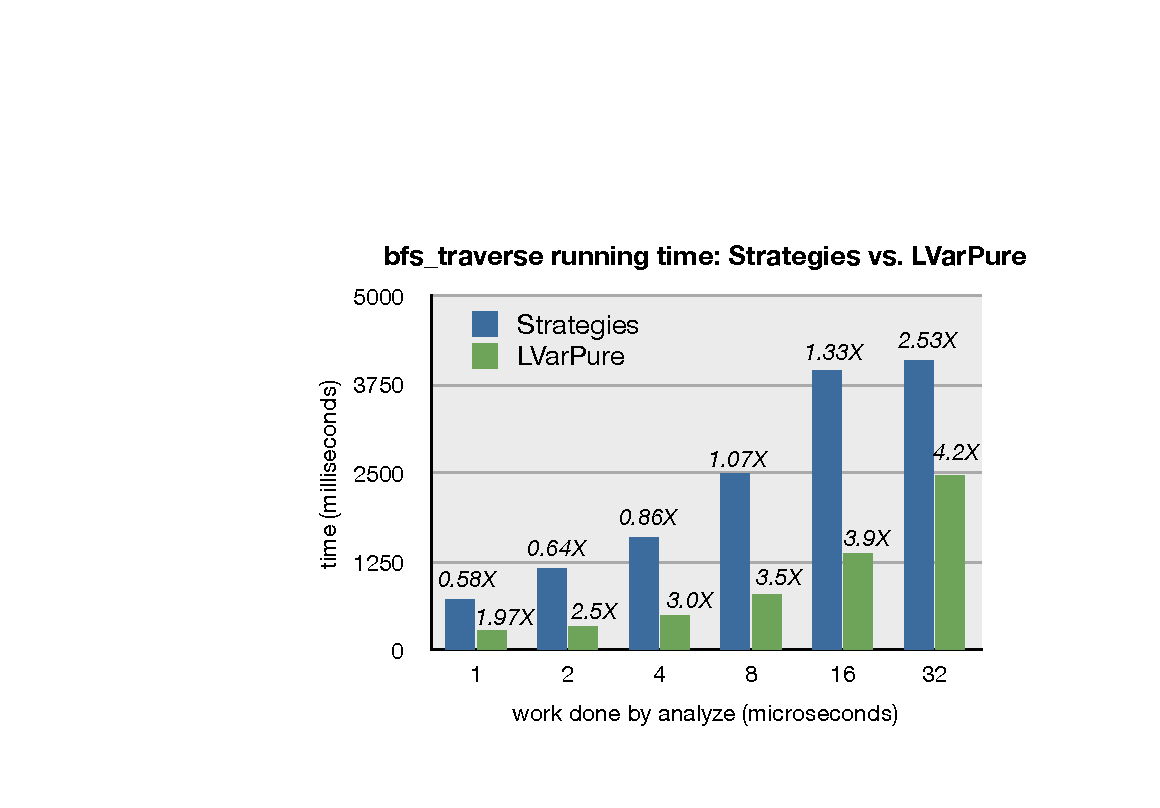
\includegraphics[width=2.5in]{figures/bargraph_with_speedups2.pdf} 
%  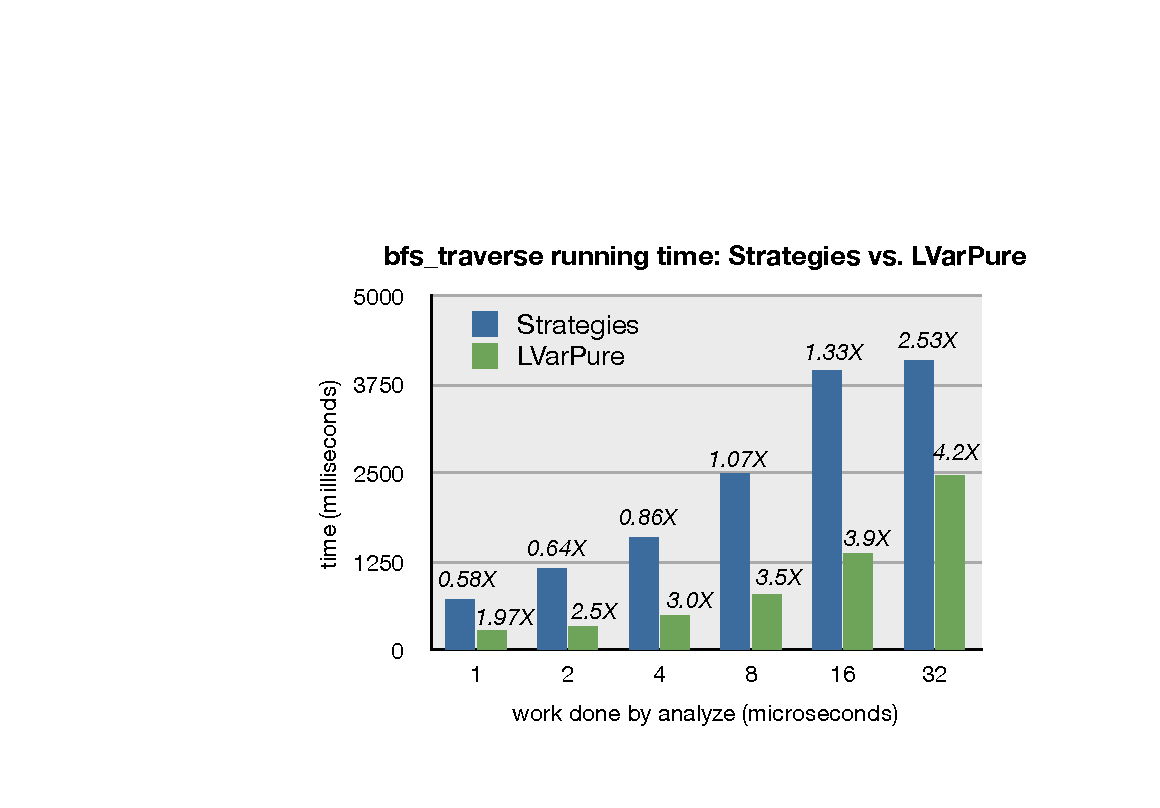
\includegraphics[width=2.7in]{figures/bargraph_with_speedups2.pdf} 

% . . side top
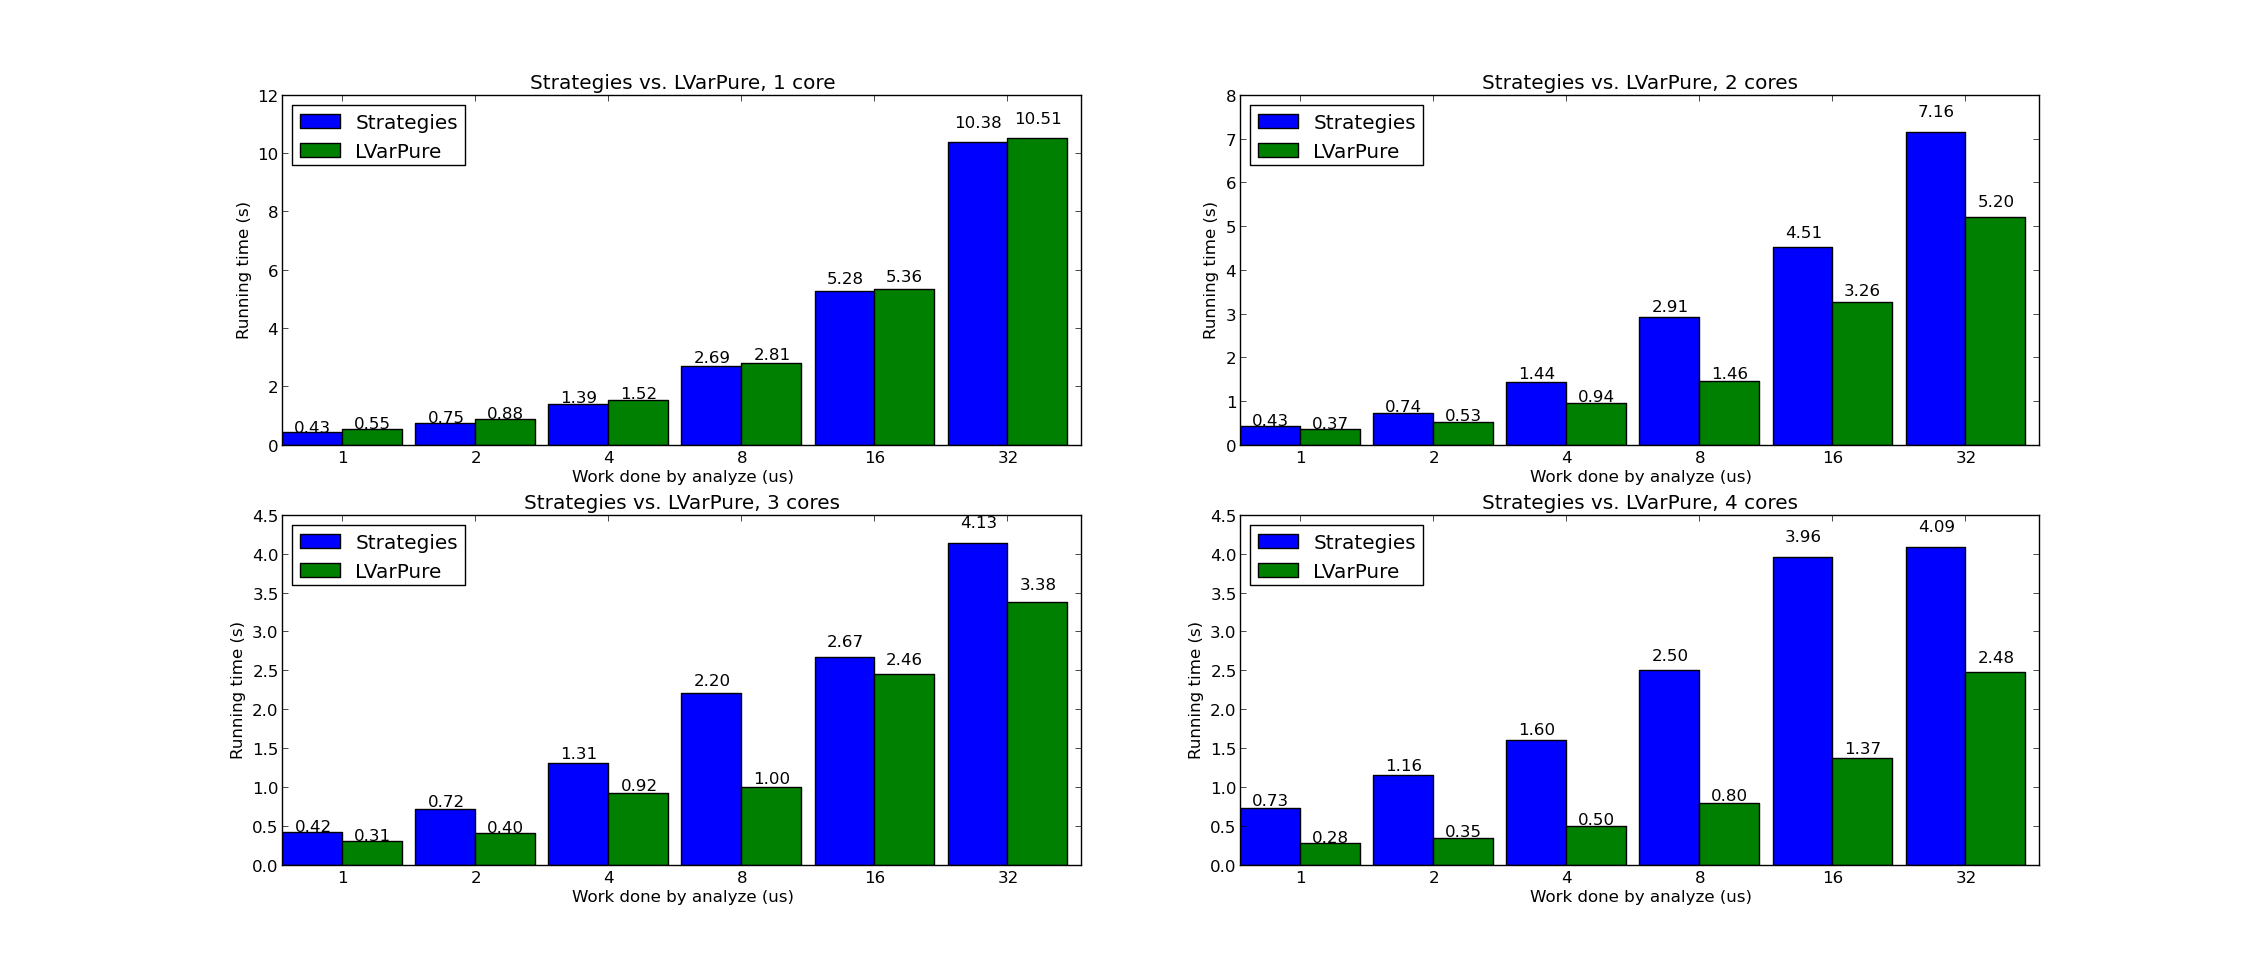
\includegraphics[clip, trim=150px 0px 0px 35px, width=7.8in, natwidth=2266px, natheight=962px]{chapter2/figures/bf_traverse_benchmark_data.png} 
\vspace{-8mm}
  \caption{\footnotesize Running time comparison of Strategies-based and LVar-based
    implementations of \lstinline|bf_traverse|, running on 1, 2, 3, and 4 cores on
    an Intel Xeon Core i5 3.1GHz (smaller is better).}
  %% \caption{\footnotesize Running time comparison of Strategies and of LVar-based
  %%   implementations of \lstinline|bf_traverse|, running on 4 cores on
  %%   an Intel Xeon Core i5 3.1GHz.  Smaller is better; numbers at top of bars indicate
  %%   parallel speedup relative to serial version of the same algorithm.}
  \label{f:performance}
\end{figure*}

%\subsection{Implementations}
\paragraph{A layered implementation}

%% \new{There are {\em three} relevant parties in deploying LVars: the 
%%   runtime implementor, the data structure author who provides an
%%   implementation for a specific lattice (\eg, a monotonically growing hashmap),
%%   and the application writer who uses LVars.  Only the application writer receives
%%   a determinism guarantee.  The data structure author uses
%%   an interface provided by the runtime implementor, who provides core functionality:
%%   thread scheduling and tracking of threads blocked on $\GET$ operations.
%% }

Use of our LVars library typically involves two parties: first, the data
structure author who uses the library directly and provides an
implementation of a specific monotonic data structure (\eg, a
monotonically growing hashmap), and, second, the application writer
who uses that data structure.  Only the application writer receives a
determinism guarantee; it is the data structure author's obligation to ensure
that the states of their data structure form a lattice and that it is only accessible via
the equivalent of $\PUT$ and $\GET$.

The data structure author uses an interface provided by our LVars library,
which provides core runtime functionality: thread scheduling and
tracking of threads blocked on $\GET$ operations.
%% We provide three implementations of our LVar library, each of which can be instantiated
%% with any lattice(s).  All three 
Concretely, 
the data structure author
imports our library
and reexports a limited interface specific to their data structure 
(\eg{}, for sets, @putInSet@ and @waitSetSizeThreshold@).  
%% Again, it is important that entire LVar runtime interface 
%% {\em not} be exported to end users of the data-structure library,
%% because if the states of the data structure do not satisfy
%% the properties of a lattice, things can go awry.  
\new{In fact, our library provides three different runtime interfaces for the data structure author
to choose among.  These ``layered'' interfaces provide the data structure author with a shifting
trade-off between the {\em ease} of meeting their proof obligation, and {\em attainable performance}:}

\begin{enumerate}
\item {\bf Pure LVars}: Here, each LVar is a single mutable
  container (an @IORef@) containing a pure value.  This requires only
  that a library writer select a purely functional data structure and
  provide a @join@\footnote{Type class
    \lstinline|Algebra.Lattice.JoinSemiLattice|.} function for it and a threshold
  predicate for each @get@ operation.  These pure functions are
  easiest to validate, for example, using the popular QuickCheck \cite{quickcheck} tool.

\item {\bf IO LVars}: Pure data structures in mutable containers
  cannot always provide the best performance for concurrent data
  structures.
% \cite{my-haskell-implementors-talk-if-there-is-space}.
  Thus we provide a more effectful interface.  With it, data
  structures are represented in terms of arbitrary mutable state; performing a
  @put@ requires an {\em update action} (@IO@) and a @get@ requires an
  effectful polling function that will be run after any @put@ to the
  LVar, to determine if the @get@ can unblock.

\item {\bf Scalable LVars}: Polling each blocked @get@ upon {\em any}
  @put@ is not very precise.  If the data structure author takes on yet more
  responsibility, they can use our third interface to reduce contention by
  managing
   the storage of blocked computations and threshold functions {\em
     themselves}.  
  For example, a concurrent set
  might store a waitlist of blocked continuations on a per-element basis,
  rather than using one waitlist for the entire LVar, as in layers (1) and (2).
\end{enumerate}

\noindent The support provided to the data structure author {\em declines} with each of
these layers, with the final option providing only parallel scheduling,
and little help with defining the specific LVar data structure.  But
this progressive cost/benefit tradeoff can be beneficial for
prototyping and then refining data structure implementations.  

% \begin{lst}
% putLV :: LVar a -> (a -> IO ()) -> Par ()
% getLV :: LVar a -> (IO (Maybe b)) -> Par b

% pure
% getLV :: LVar a -> (a -> Maybe b) -> Par b
% putLV :: JoinSemiLattice a => LVar a -> a -> Par ()

\paragraph{Revisiting our breadth-first traversal example}

In Section~\ref{section:motivation}, we proposed using LVars to
implement a program that performs a breadth-first traversal of a
connected component of a graph, mapping a function over each node in
the component.
Figure~\ref{f:bfs-lvar} gives a version of this program implemented using our LVars library.
It performs a breadth-first traversal of the 
 @profiles@ graph with effectful $\PUT$
operations on a shared set variable.  
\new{This variable, \lstinline|analyzedSet|, has to be modified
multiple times by \lstinline|putInSet| and thus cannot be an IVar.\footnote{Indeed, there are
  subtle problems with encoding a set even as a linked structure of
  IVars.  For example, if it is represented as a tree, who writes the root?}  The callback function
 \lstinline|analyze| is ``baked into'' \lstinline|analyzedSet| and may run
  as soon as new elements are inserted.  
  %% (In the $\lambdaLVar$ calculus,
  %% \lstinline|analyze| could be built into the $\REIFY$ function
  %% and applied to the result of $\GET$.)
}
Our implementation uses the ``Pure LVars'' runtime layer described above: 
@analyzedSet@ is nothing more than a tree-based data structure
(@Data.Set@) stored in a mutable location.  

\paragraph{Preliminary benchmarking results}

We compared the performance of the LVar-based implementation of @bf_traverse@ against the version in Figure~\ref{f:bfs-pure}, which we ran using the 
\\ @Control.Parallel.Strategies@ library
\cite{marlow-par}, version 3.2.0.3. (\new{Despite being a simple algorithm, even breadth-first search by itself
is considered a useful benchmark; in fact, the well-known
``Graph 500'' \cite{graph500} benchmark is exactly breadth-first search.})

We evaluated the Strategies and LVar versions of @bf_traverse@
by running both on a local random directed graph of 40,000 nodes and
320,000 edges (and therefore an average degree of 8), simulating the
@analyze@ function by doing a specified amount of work for each node,
which we varied from 1 to 32 microseconds.
Figure \ref{f:performance} shows the results of our evaluation on 1, 2, 3, and 4 cores.
Although both the Strategies and LVar versions enjoyed a
 speedup as we added parallel resources, the LVar
version scaled particularly well.
A subtler, but interesting point is that, in the Strategies version,
it took an average of 64.64 milliseconds for the first invocation of
@analyze@ to begin running after the program began, whereas in the
LVar version, it took an average of only 0.18 milliseconds,
indicating that the LVar version allows work to be
pipelined.



\rnote{Report time-to-first-f results in prose I suppose....}


%% \lk{Shouldn't stuff like this be pushed to an evaluation section
%%   further along in the paper?  Not sure it belongs right in the
%%   intro.}
%% \new{In fact, we know it is possible to implement these data structures even more
%% efficiently.  The key question addressed in this paper, is not whether
%% such a system can be implemented, but:}
%The question then becomes: 
%% {\em how might we convince ourselves that every program
%% written with such a library is deterministic, especially when mixing different
%% data structures?}
%% \rn{TODO: More explicitly declare here that the paper is not about this
%%   implementation, but about the underlying theory.}
%
%% The existence of, and usefulness of, practical implementations motivates
%% us to pursue this question.


